\documentclass[../main.tex]{subfiles} 
\usepackage{ctex}
\usepackage{xltxtra}
\usepackage{graphicx}
\usepackage{booktabs}
\usepackage{amsmath}
\usepackage{mathdots}
\usepackage{amssymb}
\usepackage{cite}
\usepackage{appendix}
\usepackage{array}
\usepackage{subfigure}
\begin{document}

    \subsection{缺失值填充}

        \subsubsection{缺失值观察及特征填充}

        在之前的数据浏览时已经发现训练集和测试集的特征中,除了PassengerId特征其他各个特征都存在缺失,在此对于各个特征缺失量进行统计,可以发现每个特征的缺失量都在3\%左右,但是有缺失值的数据超过了20\%,如图17所示。因此,不能简单的采用丢弃的方法,必须要给各维度数据进行填充。

        \begin{figure}[H]
            \centering
            \subfigure[不同特征缺失值数量]
            {
                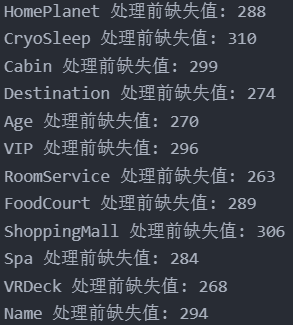
\includegraphics[scale=0.5]{Sec3_1.png}
            }
            \subfigure[总数据缺失值数量]
            {
                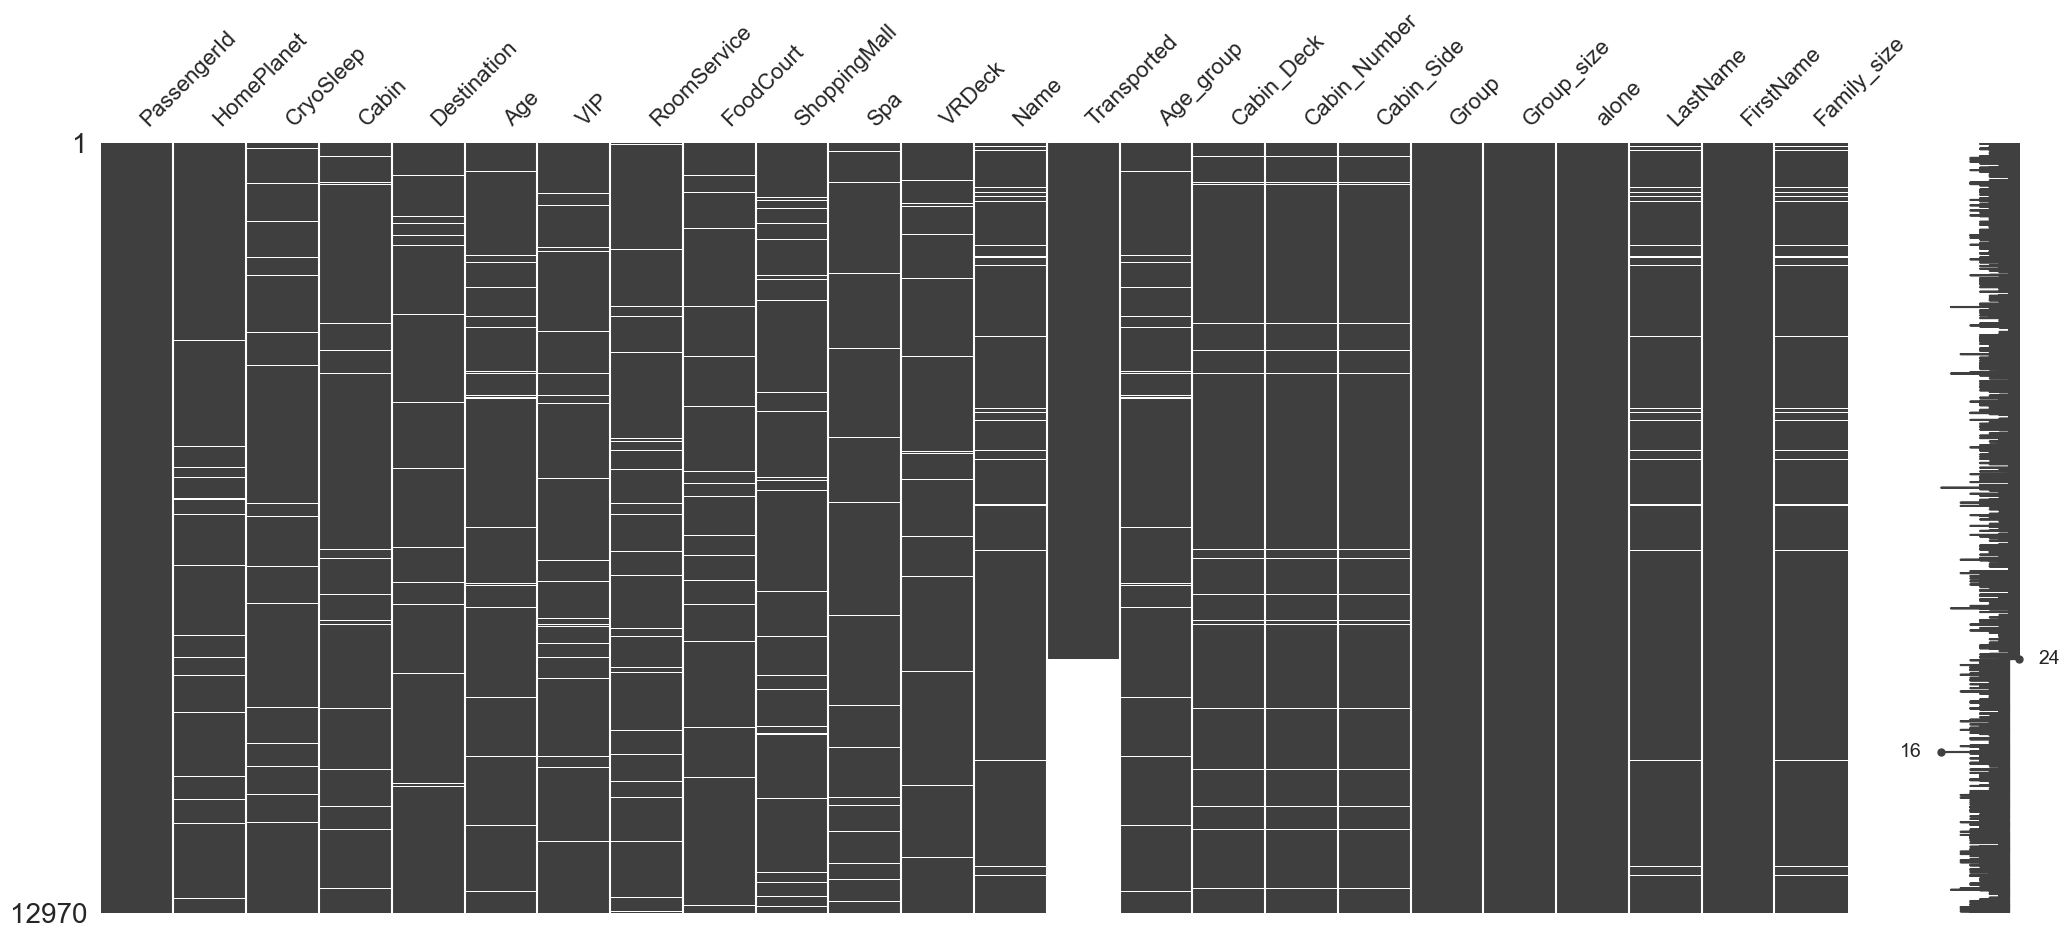
\includegraphics[scale=0.2]{Sec3_2.png}
            }
            \caption{缺失值}
        \end{figure}

        首先先将训练集和测试集进行合并,一同处理。其次对于年龄将其分成6个组别,分别为"Age\_0-12","Age\_13-17","Age\_18-25","Age\_26-30","Age\_31-50","Age\_51+",不同年龄段人数如图18所示。
        并且如前文所说,对于Cabin进行拆分,得到Cabin\_Deck,Cabin\_Number,Cabin\_Side三个特征;对于PassengerId特征进行拆分得到Group特征,并且根据Group人数得到Group\_size和alone两个特征;
        对于Name特征进行拆分为First Name和Last Name,并且利用Last Name特征得出Family Size特征,因为从Last Name可以帮助判断是否乘客是同一家族的,这和Group的概念一样,可以判断不同乘客是否一起旅行。

        \begin{figure}[H]
            \centering
            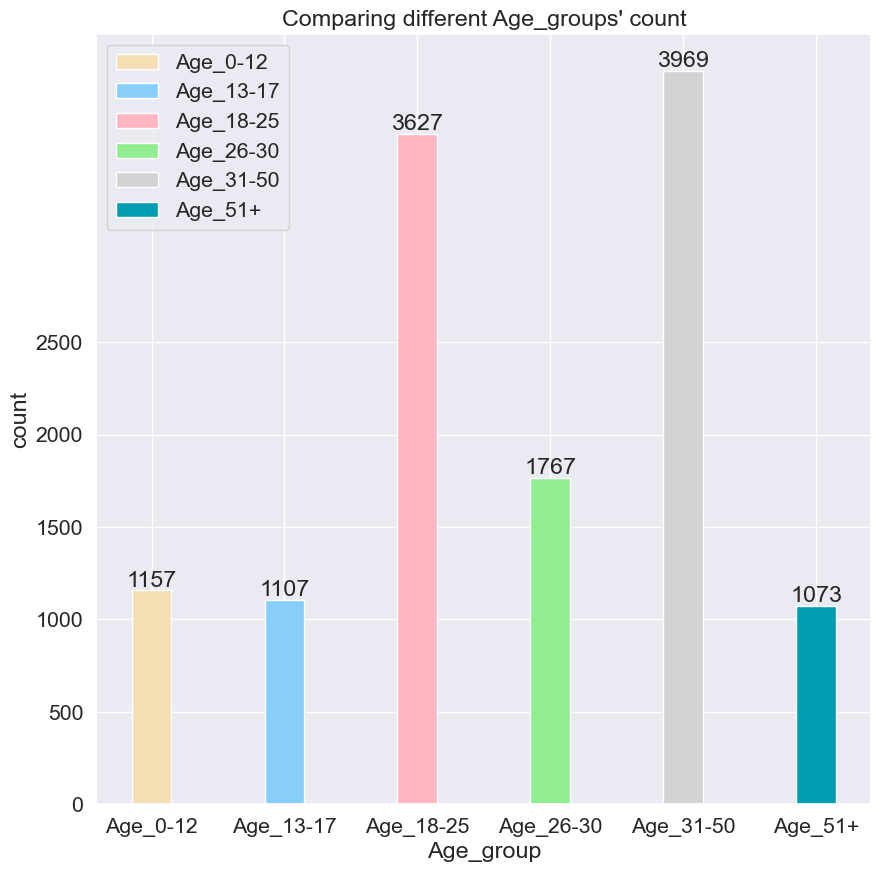
\includegraphics[scale=0.3]{Sec3_3.png}
            \caption{年龄分组对比}
        \end{figure}

        \subsubsection{缺失值填充}

            首先填充的是HomePlanet特征,由PassengerId的叙述中得知同一Group的乘客很有可能一同旅行,因此利用Group处理HomePlanet特征。
            因此,统计不同Group中每个乘客的HomePlanet并绘制成折线图,可以发现:同一Group中的乘客都来自同一个HomePlant,如图19.(a)所示。
            因此可以利用该信息进行填充。

            同时在之前的数据分布可视化的过程中,发现Cabin\_Deck和HomePlanet可能存在关系,因此利用热力图画出不同Cabin\_Deck中来自各个HomePlanet的乘客数量,如图19.(c)所示。
            可以发现,当乘客的桌子为A, B, C , T时,HomePlanet为Europa;乘客的桌子为G时,母星为Earth;乘客的桌子为D, E, F时母星较为复杂。

            Last Name相同的乘客应该来自同一家族,和Group的概念相同,利用折线图可以发现:同一LastName的乘客都来自同一个HomePlanet,如图19.(b)所示。

            在进行了3次填充后,发现还剩下10条数据缺失,查看10条数据可以发现Cabin\_Deck都是D或F。又因为Cabin\_Deck,HomePlanet和Destination应有很强的相关性,所以查看这十条数据的Destination发现都是TRAPPIST-1e。
            最后利用热力图查看不同HomePlanet中前往各个Destination的乘客数量,可以发现:前往TR的人大多数来自Earth,但是桌子为D的人来自Mars和Europa(Mars比例高),而桌子为F的人来自Earth和Mars(Earth比例高),如图19.(d)所示。
            因此对于Deck为D的乘客,填充其HomePlanet为Mars,而Deck为F的乘客,填充其HomePlanet为Earth。

            \begin{figure}[H]
                \centering
                \subfigure[Group与HomePlanet]
                {
                    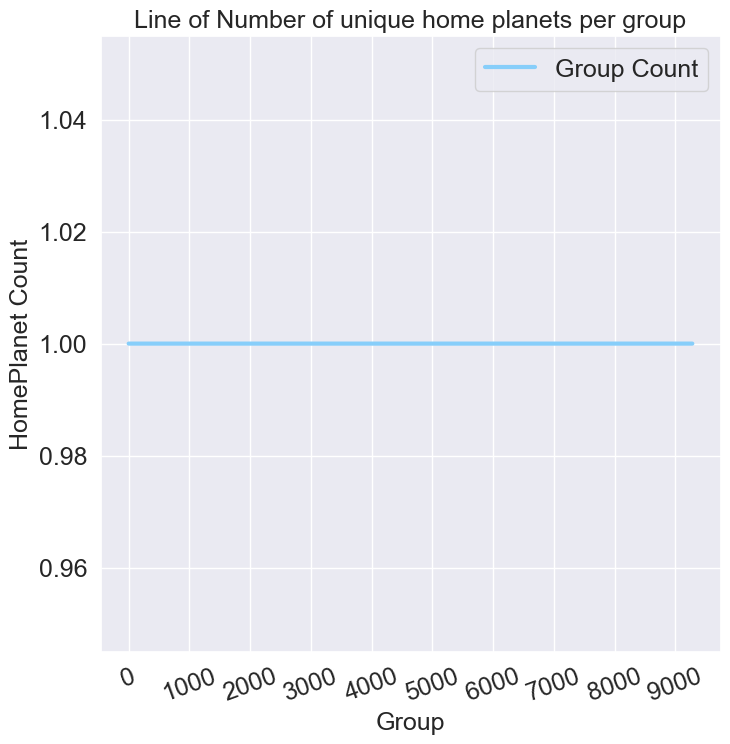
\includegraphics[scale=0.3]{Sec3_4.png}
                }
                \subfigure[LastName与HomePlanet]
                {
                    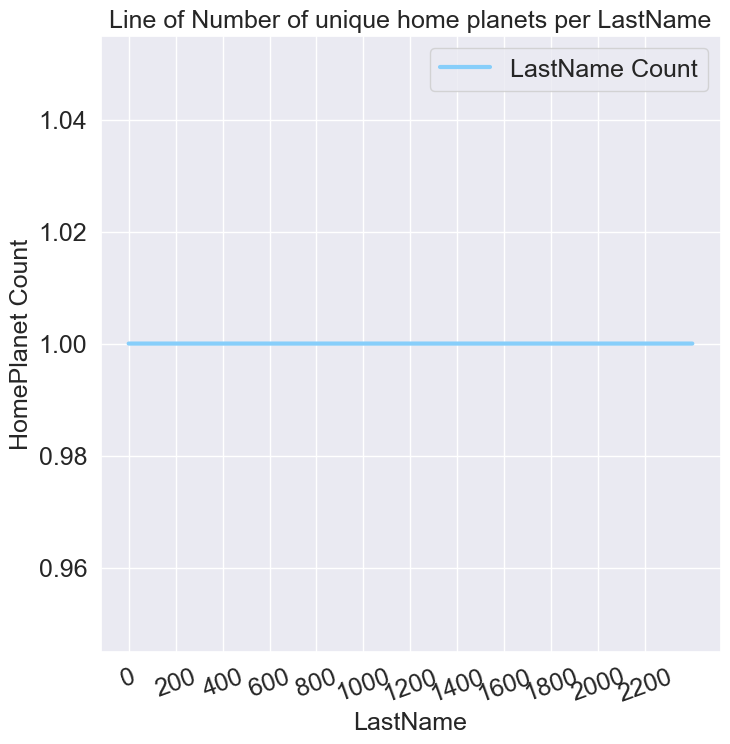
\includegraphics[scale=0.3]{Sec3_6.png}
                }
                
                \subfigure[Cabin\_Deck与HomePlanet]
                {
                    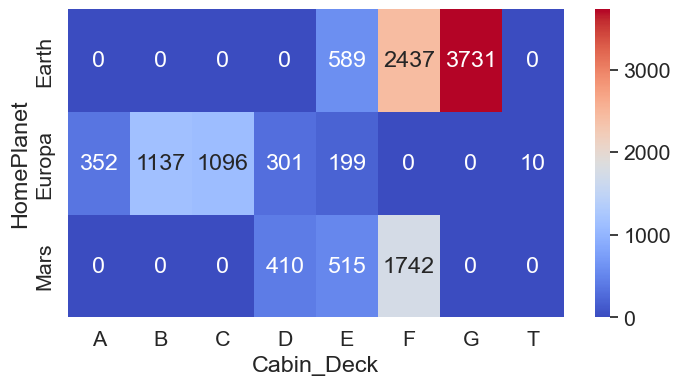
\includegraphics[scale=0.4]{Sec3_5.png}
                }
                \subfigure[Destination与HomePlanet]
                {
                    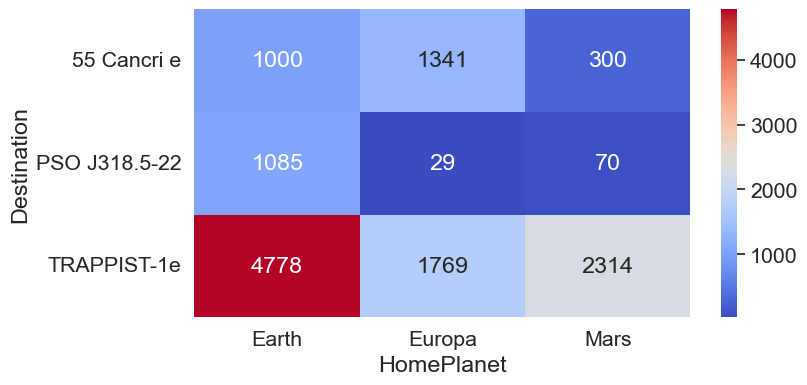
\includegraphics[scale=0.4]{Sec3_7.png}
                }
                \caption{HomePlanet}
            \end{figure}

            其次查看的是Destination特征,由于之间所认识到的Group、LastName、HomePlanet的相关性,因此用了同样的观察方法观察Group、LastName与Destination之间的关系。
            但是可以发现这两者与Destination并没有太大的联系,如图20.(a)和图20.(b)所示。
            这时候剩下可以使用的信息只有Cabin\_Deck与Destination之间的关系,因此利用热力图绘制出同一Cabin\_Deck中前往不同Destination的乘客数,可以发现除了DeckA前往55和TR的乘客人数较为相近外,其他Deck前往TR的人数都远远超过其他Deck,如图20.(c)所示。
            因此我们可以利用众数思想,将这些Destination缺失的乘客都赋值为TRAPPIST-1e.

            \begin{figure}[H]
                \centering
                \subfigure[Group与Destination]
                {
                    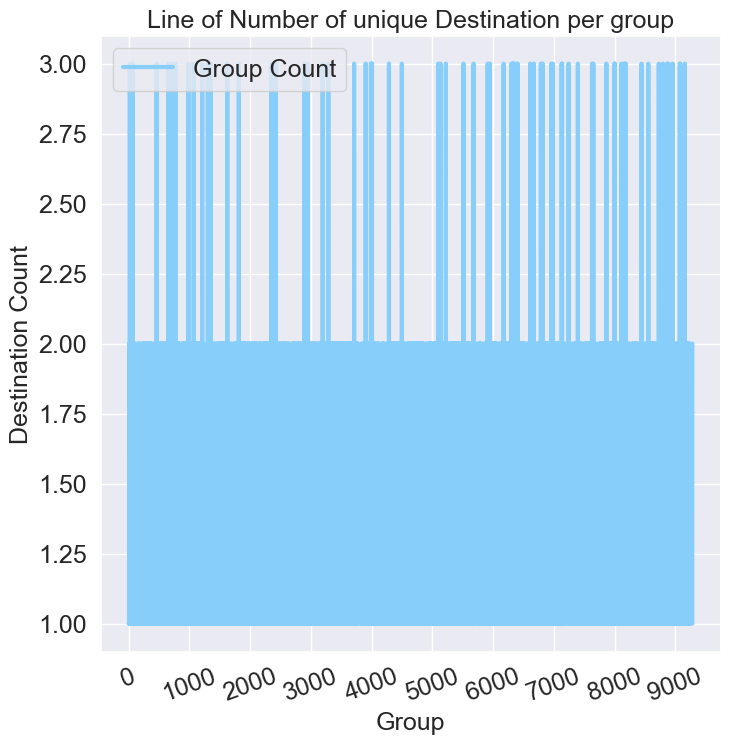
\includegraphics[scale=0.3]{Sec3_8.png}
                }
                \subfigure[LastName与Destination]
                {
                    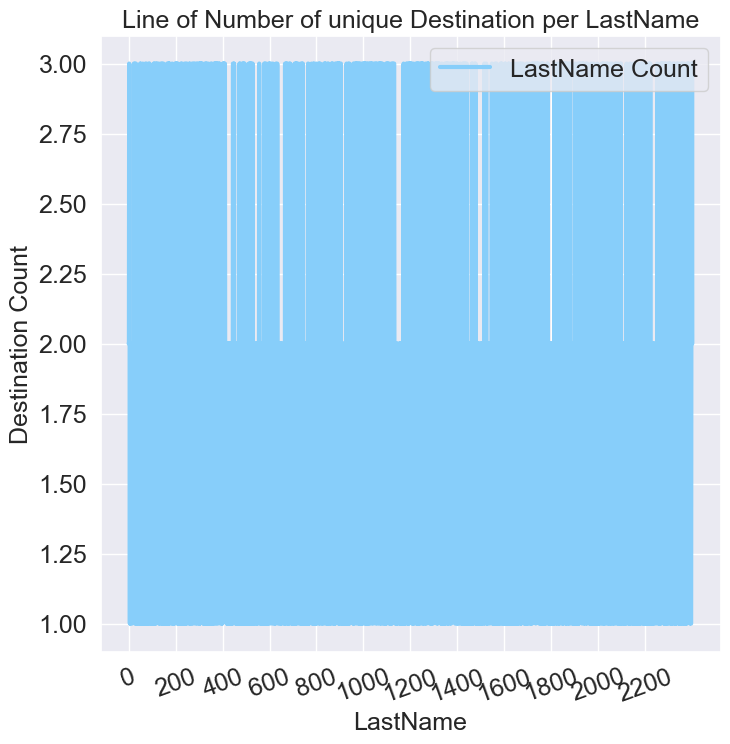
\includegraphics[scale=0.3]{Sec3_9.png}
                }
                
                \subfigure[Cabin\_Deck与Destination]
                {
                    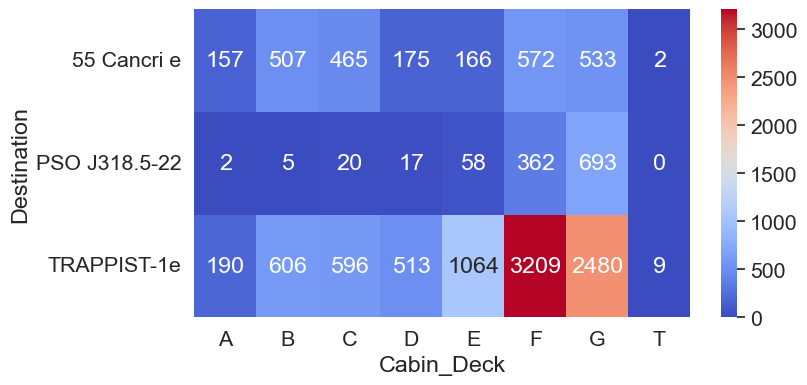
\includegraphics[scale=0.4]{Sec3_10.png}
                }
                \caption{Destination}
            \end{figure}

            接着填充的是LastName特征。由于LastName和Group有很强的相关性,而Group\_Size是由Group引出的特征,因此LastName和Group\_Size有很强的相关性。因此,利用折线图,观察Group\_Size大于1的Group中各个成员的LastName是否相同,如图21所示。
            可以发现超过80\%的Group中只有一种LastName,因此对于同一Group的乘客可以赋予同一LastName。

            \begin{figure}[H]
                \centering
                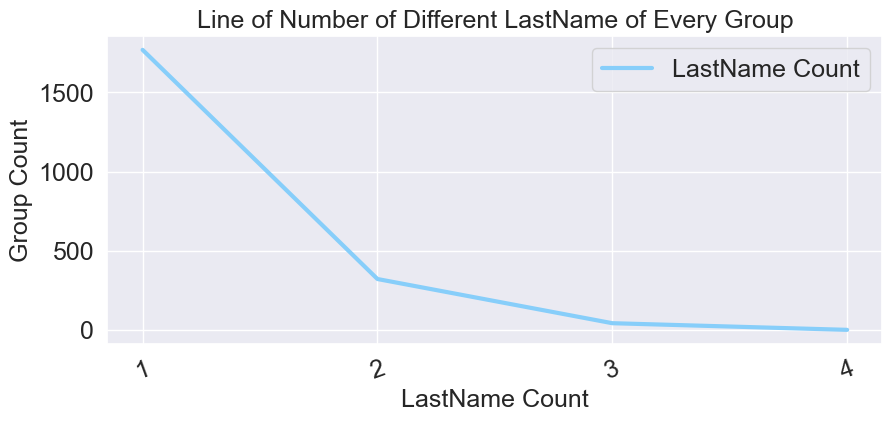
\includegraphics[scale=0.3]{Sec3_11.png}
                \caption{LastName和Group\_Size}
            \end{figure}

            对于剩下的LastName缺失值采用随机选取方法,而缺失的FirstName由于和所有特征都没有什么关系,因此FirsttName直接使用Random进行选取,并将FirstName和LastName进行组合重新赋值给Name。

            继续填充的是Cabin特征。利用折线图分别绘制Cabin\_Deck、Cabin\_Number、Cabin\_Side三个特征在Group\_Size大于1的时候,每个Group中出现的数量,如图22所示。
            可以发现同一个Group的成员都在同一个Cabin\_Side上,而Cabin\_Deck和Cabin\_Number也有超过70\%的Group只有一种取值。因此首先利用相同Group成员的Cabin\_Side填充缺失的Cabin\_Side。

            \begin{figure}[H]
                \centering
                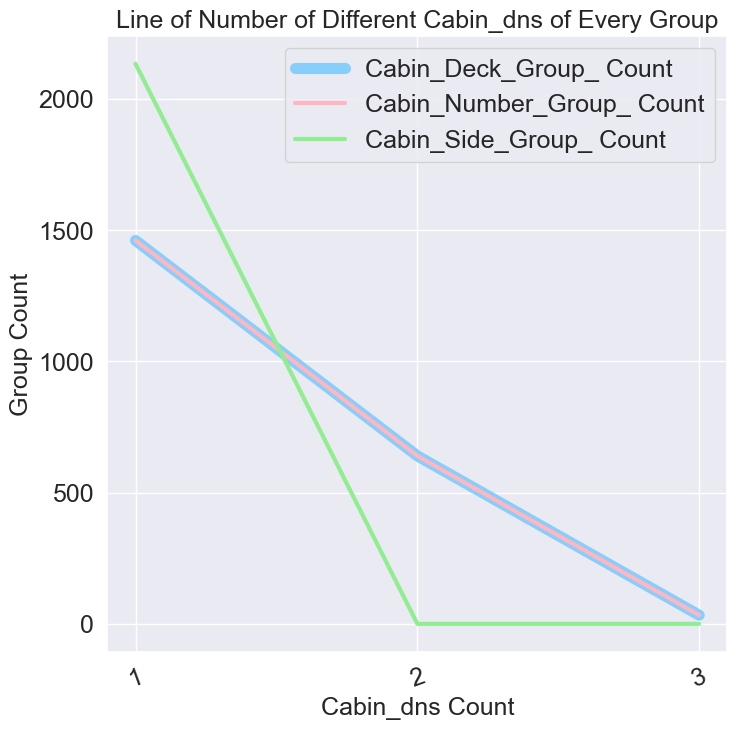
\includegraphics[scale=0.4]{Sec3_12.png}
                \caption{Group Count和Cabin\_Deck、Cabin\_Number、Cabin\_Side数量}
            \end{figure}

            处理完后查看Cabin\_Side中S和P的数量,可以发现两者几乎为1:1的关系,因此剩下的值采用Random的方法直接填补。

            同样的对于Cabin\_Deck,可以认为同一Group的乘客坐在同一个Cabin\_Deck上,因此对于位于只有一种Cabin\_Deck取值的Group中缺失乘客的Cabin\_Deck,利用同一Group中的其他成员的Cabin\_Deck填充。

            又由之前的信息可以得知,Cabin\_Deck和HomePlanet及Destination有较强的关系,如图23所示。
            列出表格查看后可以发现:来自Mars的大多数坐F,来自Earth的大多数坐F或G,来自Europa的大多数坐B或C。

            \begin{figure}[H]
                \centering
                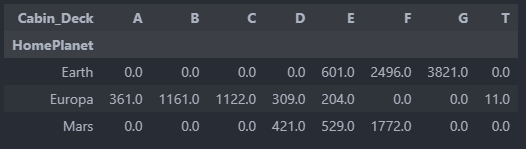
\includegraphics[scale=0.5]{Sec3_13.png}
                \caption{HomePlanet和Cabin\_Deck}
            \end{figure}

            而对于Cabin\_Number,由于可取数值过多,并且数据之间没有太多关系,因此直接采用Random随机填充。

            对于VIP特征,由之前的VIP特征分析可知,超过95\%乘客都不是VIP,因此对于VIP特征缺失的乘客,可以直接使用众数填充为False。

            对于Age特征,该特征应该和很多特征相关,比如说是否消费,是否是一个人旅行,而如果不是一个人旅行,证明Group这个特征非常重要,Group又与Cabin\_Deck和HomePlanet有很强的关系。
            因此首先新建立特征spending代表乘客是否消费,其次根据HomePlanet,spending,alone,Cabin\_Deck和Age这几个特征进行制表,取满足这些条件下的乘客Age的中位数为表中数字,如图24所示。
            并根据表中数字和满足的关系对于缺失Age特征的乘客进行特征。

            \begin{figure}[H]
                \centering
                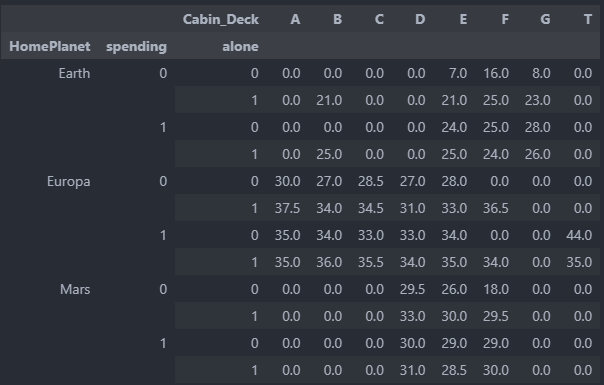
\includegraphics[scale=0.4]{Sec3_14.png}
                \caption{Age}
            \end{figure}

            对于CryoSleep特征,按照我们日常生活中的习惯来说,乘客是否休眠,主要查看的就是乘客是否有花费,为了进一步确定该想法是否正确,根据CryoSleep和spending特征进行制表并查看,如图25所示。
            可以发现,只要有花费,就是处于不休眠的状态,而超过85\%的没有花费的乘客都是处于休眠状态,因此可以简单地根据乘客是否有花费来判断乘客的CryoSleep特征。

            \begin{figure}[H]
                \centering
                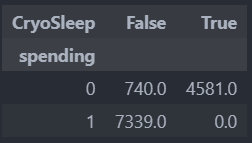
\includegraphics[scale=0.6]{Sec3_15.png}
                \caption{CryoSleep和sleeping}
            \end{figure}

            同理对于五个代表消费的特征RoomService,FoodCourt,ShoppingMall,Spa,VRDeck,只要乘客处于休眠状态即可认为五项消费均为0.
            而对于其他不处于休眠状态而消费特征依然缺失的乘客,可以很自然地想到,消费应该与不同年龄段、是否一个人出行、生活环境相关。
            因此可以根据HomePlanet、alone、Age\_group和RoomService,FoodCourt,ShoppingMall,Spa,VRDeck进行制表,如图26.(a)、(b)、(c)、(d)、(e)所示,并使用均值进行缺失值填补。

            \begin{figure}[H]
                \centering
                \subfigure[RoomService]
                {
                    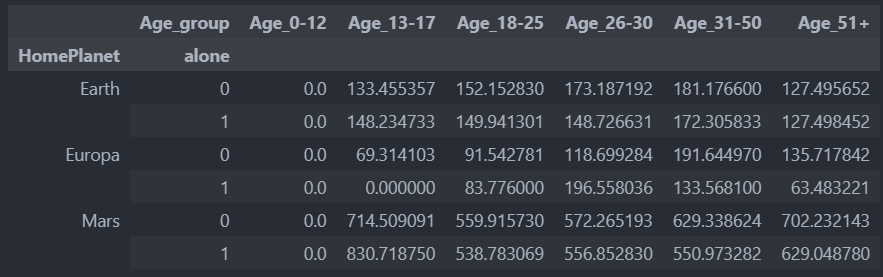
\includegraphics[scale=0.4]{Sec3_16.png}
                }
                \subfigure[FoodCourt]
                {
                    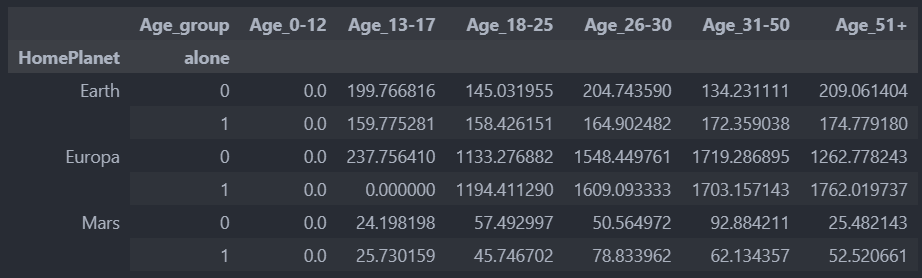
\includegraphics[scale=0.4]{Sec3_17.png}
                }
                
                \subfigure[ShoppingMall]
                {
                    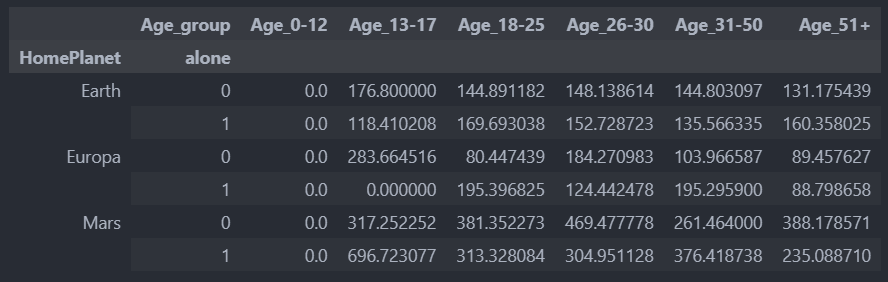
\includegraphics[scale=0.4]{Sec3_18.png}
                }
                \subfigure[Spa]
                {
                    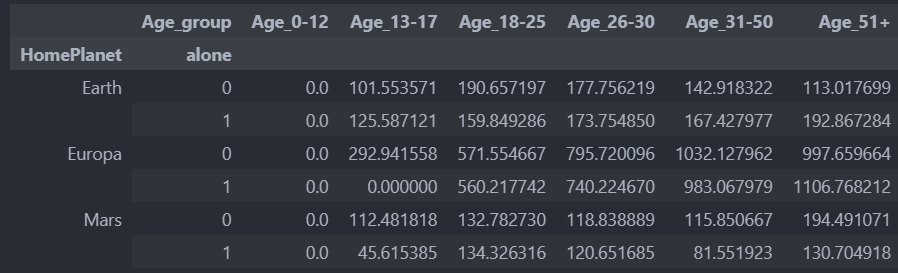
\includegraphics[scale=0.4]{Sec3_19.png}
                }

                \subfigure[VRDeck]
                {
                    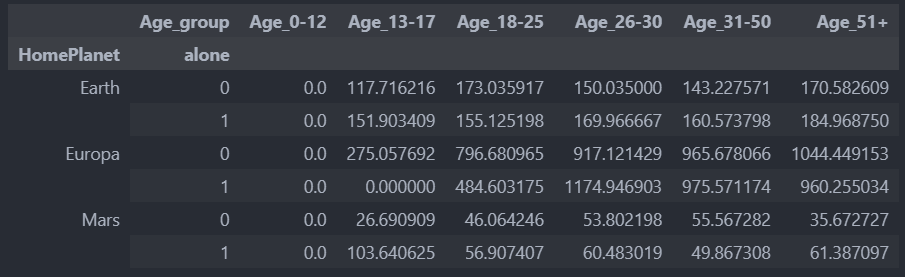
\includegraphics[scale=0.4]{Sec3_20.png}
                }
                \caption{Expenditure}
            \end{figure}

            最后进行Family Size特征的更新,至此,缺失值全部填充完毕。

    \subsection{数据变换}

        \subsubsection{特征变换}

            对于连续变量Age进行离散化,为Age\_group,前文已经叙述过,并且画出了分布图,在这里不再进行重复,补充一张填补缺失值后的Age\_group分布图,如图27所示。

            \begin{figure}[H]
                \centering
                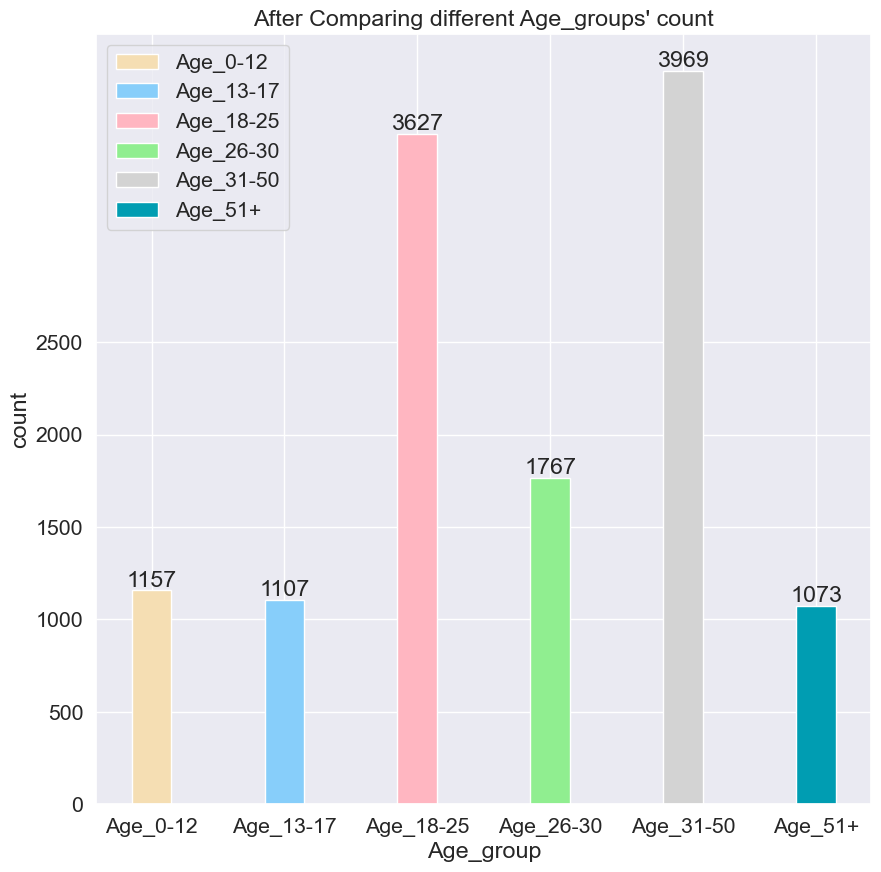
\includegraphics[scale=0.5]{Sec3_21.png}
                \caption{Age\_group(after)}
            \end{figure}

            对于五个代表消费的特征RoomService,FoodCourt,ShoppingMall,Spa,VRDeck,数据值从0到几万不止,数据差别很大,使得整个样本偏差变大,尝试对数变换,sigmoid变换减小偏差。
            可以看出,如果使用sigmoid变换,虽然数值成功归一化了,但是无法体现出太大的差异性,不利于模型的学习,因此使用对数变换。变换结果如图28所示。

            \begin{figure}[H]
                \centering
                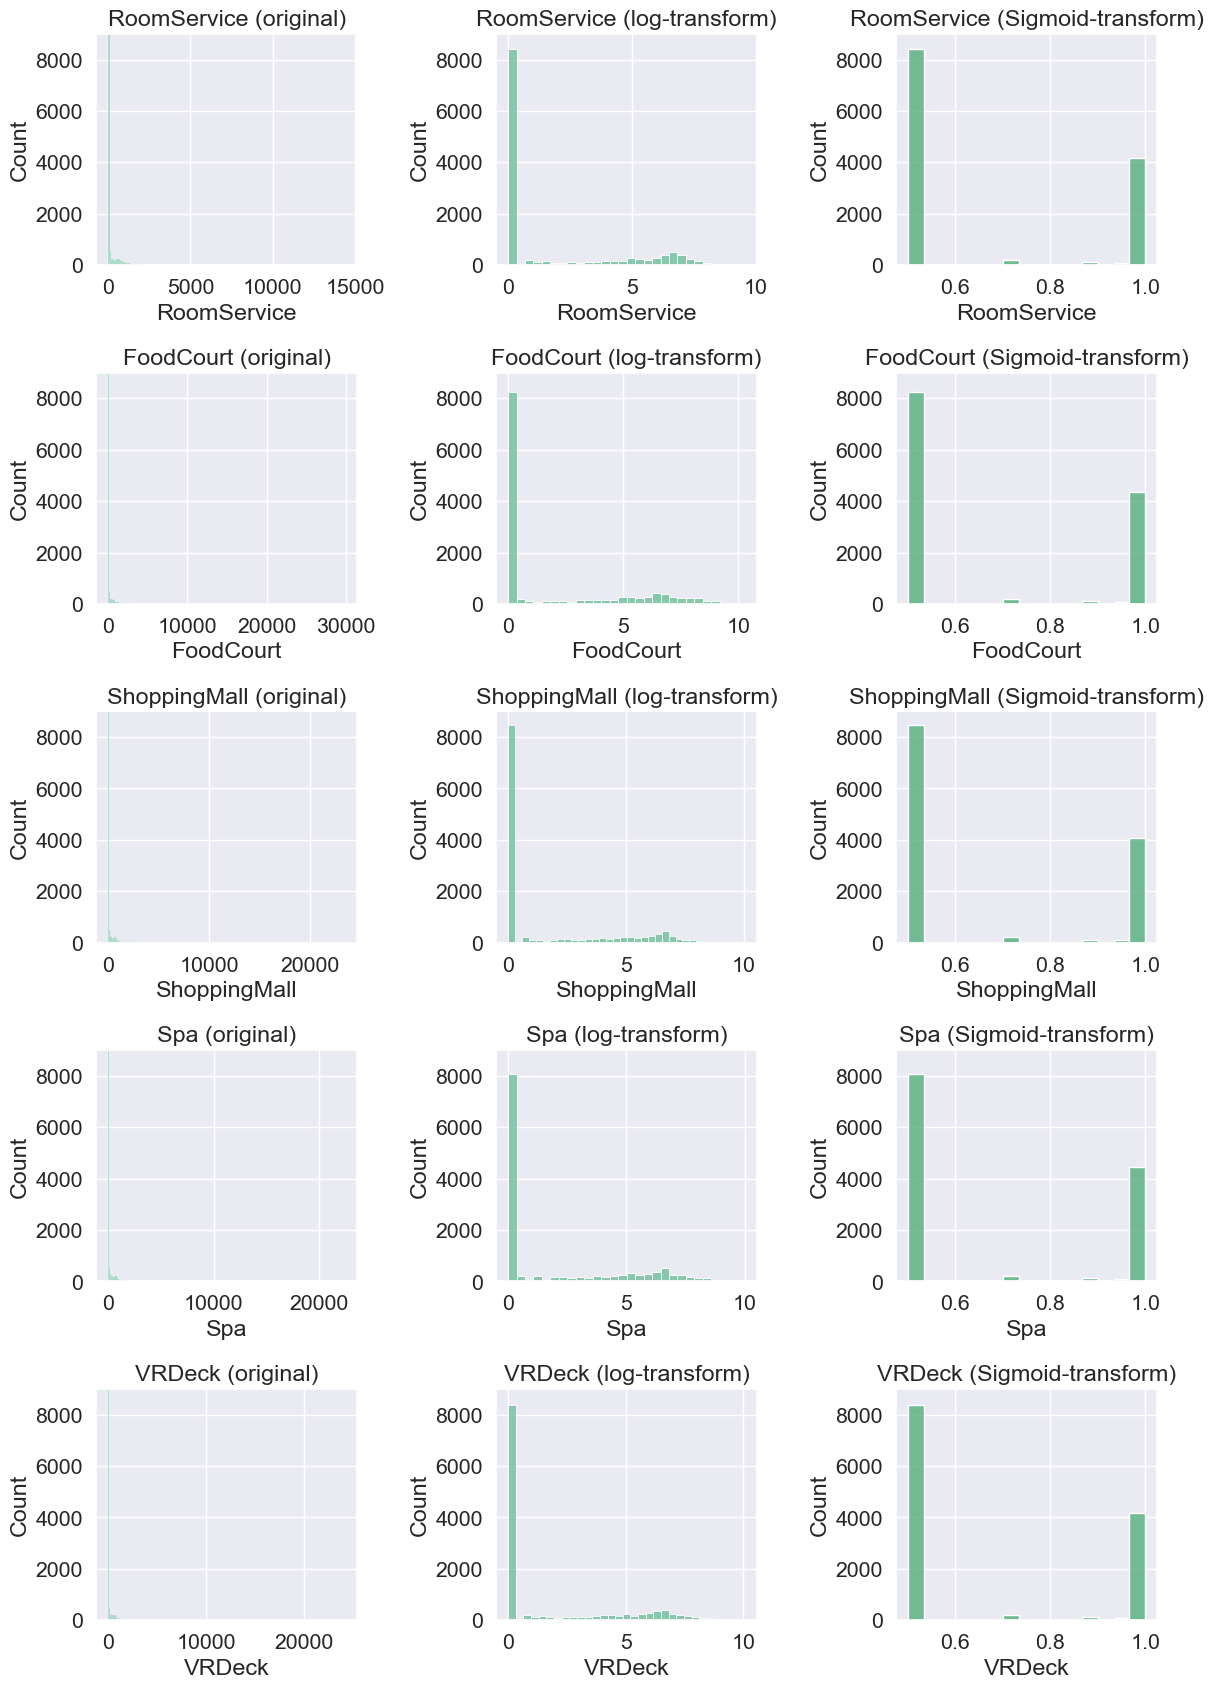
\includegraphics[scale=0.4]{Sec3_22.png}
                \caption{Expenditure Transform}
            \end{figure}

        \subsubsection{特征编码}

            最后利用是否有标签Transported重新划分出训练集和预测集。
            
            由于算法只能接收数值型数据的输入,而不能是字母或单词,所以必须先将Object形式的数据转换成数值型数据。利用sklearn.preprocessing中的LabelEncoder函数进行编码,编码后的训练集部分数据如图29所示,编码后部分特征格式如表2,3,4所示。

            \begin{figure}[H]
                \centering
                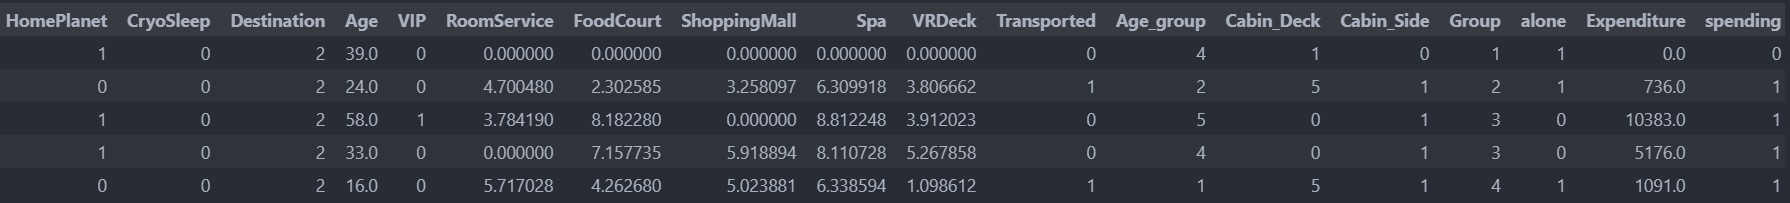
\includegraphics[scale=0.4]{Sec3_23.png}
                \caption{Encoder Data}
            \end{figure}

            \begin{table}[H]
                \footnotesize
                \centering
                \begin{tabular}{|c|ccc|cc|ccc|cc|}
                \hline
                \textbf{Feature} & \multicolumn{3}{c|}{\textbf{HomePlanet}}                        & \multicolumn{2}{c|}{\textbf{CryoSleep}} & \multicolumn{3}{c|}{\textbf{Destination}}                                            & \multicolumn{2}{c|}{\textbf{Transported}}  \\ \hline
                \textbf{Data}    & \multicolumn{1}{c|}{Earth} & \multicolumn{1}{c|}{Europa} & Mars & \multicolumn{1}{c|}{False}    & True    & \multicolumn{1}{c|}{55 Cancri e} & \multicolumn{1}{c|}{PSO J318.5-22} & TRAPPIST-1e  & \multicolumn{1}{c|}{False}     & True      \\ \hline
                \textbf{Encode}  & \multicolumn{1}{c|}{0}     & \multicolumn{1}{c|}{1}      & 2    & \multicolumn{1}{c|}{0}        & 1       & \multicolumn{1}{c|}{0}           & \multicolumn{1}{c|}{1}             & 2            & \multicolumn{1}{c|}{0}         & 1         \\ \hline
                \end{tabular}
                \caption{部分数据编码}
            \end{table}


            \begin{table}[H]
                \centering
                \footnotesize
                \begin{tabular}{|c|cccccc|cc|}
                \hline
                \textbf{Feature} & \multicolumn{6}{c|}{\textbf{Age\_group}}                                                                                                                                           & \multicolumn{2}{c|}{\textbf{VIP}} \\ \hline
                \textbf{Data}    & \multicolumn{1}{l|}{Age\_0-12} & \multicolumn{1}{l|}{Age\_13-17} & \multicolumn{1}{l|}{Age\_18-25} & \multicolumn{1}{l|}{Age\_26-30} & \multicolumn{1}{l|}{Age\_31-50} & Age\_51+  & \multicolumn{1}{c|}{False} & True \\ \hline
                \textbf{Encode}  & \multicolumn{1}{l|}{0}         & \multicolumn{1}{l|}{1}          & \multicolumn{1}{l|}{2}          & \multicolumn{1}{l|}{3}          & \multicolumn{1}{l|}{4}          & 5         & \multicolumn{1}{c|}{0}     & 1    \\ \hline
                \end{tabular}
                \caption{Age\_group和VIP编码}
            \end{table}

            \begin{table}[H]
                \centering
                \footnotesize
                \begin{tabular}{|c|cccccccc|cc|}
                \hline
                \textbf{Feature} & \multicolumn{8}{c|}{\textbf{Cabin\_Deck}}                                                                                                                                        & \multicolumn{2}{c|}{\textbf{Cabin\_Side}} \\ \hline
                \textbf{Data}    & \multicolumn{1}{c|}{A} & \multicolumn{1}{c|}{B} & \multicolumn{1}{c|}{C} & \multicolumn{1}{c|}{D} & \multicolumn{1}{c|}{E} & \multicolumn{1}{c|}{F} & \multicolumn{1}{c|}{G} & T & \multicolumn{1}{c|}{P}         & S        \\ \hline
                \textbf{Encode}  & \multicolumn{1}{c|}{0} & \multicolumn{1}{c|}{1} & \multicolumn{1}{c|}{2} & \multicolumn{1}{c|}{3} & \multicolumn{1}{c|}{4} & \multicolumn{1}{c|}{5} & \multicolumn{1}{c|}{6} & 7 & \multicolumn{1}{c|}{0}         & 1        \\ \hline
                \end{tabular}
                \caption{Cabin\_Deck和Cabin\_Side编码}
            \end{table}

\end{document}